\section{Experiments}
\label{sec:experiments}
In this section we try to answer the following research questions: 
\begin{enumerate}
  \item Can KPCNet generate more specific CQs than previous baselines? 
  \item To what extent can we control the generation of KPCNet by operating on the keywords with methods like keyword selection and filtering (\S \ref{sec:selection}, \S \ref{sec:probing}) ?
  \item How well can our proposed keyword selection methods promote local diversity, compared to existing diverse generation approaches?
\end{enumerate}

\subsection{Evaluation metrics}
Most previous works on question 
generation~\citep{jain2017creativity, hu2018aspect, rao2019answer} 
adopts \textit{Individual-level} evaluation protocol, where only the best generated question of a group is evaluated (thus also named \textit{Oracle} metrics). Specially, for proper evaluation of the novel \textit{Diverse CQGen} task, we need to evaluate the overall quality and diversity of CQ groups. We refer to this as \textit{Group-level} evaluation. We adopt automatic metrics as well as human judgements on both level. 

\subsubsection{Automatic Metrics}
We use \textbf{Distinct-3} (DIVERSITY), 
\textbf{BLEU}
\footnote{\url{https://github.com/moses-smt/mosesdecoder/blob/master/scripts/generic/multi-bleu.perl}}
%\ZL{Must keep this for reproducibility, because there are multiple different versions of BLEU.}
\citep{papineni2002bleu} and 
\textbf{METEOR} \citep{banerjee2005meteor} for individual-level automatic evaluation.
For group-level evaluation, we adopt the evaluation protocol proposed by \citet{shen2019mixture} for diverse machine translation, and use \textbf{Pairwise-BLEU} and \textbf{Avg BLEU} as the evaluation metric. We report them in percentage.
\subsubsection{Human Judgements}
For individual-level human judgements, we show every annotator one context and one generated question for each system (including reference). The system name is invisible to the annotator and the order is randomly shuffled. The selected candidate is the one that achieved the highest BLEU in the generation group. 
We ask human to judge the \textbf{Grammaticality(G), Relevance(R), Seeking New Information(N) and Specificity(S)} of the questions. Also, noting that the system generations are also prone to make logical errors like improper repetition (``does the lid have a lid ?'') or asking for relevant but not exactly the correct object (asking ``what is the thickness of the bed ?'' for a mattress), we further judge the \textbf{Logicality(L)} of the candidate. Futher descriptions of these metrics can be found in Appendix B.

For group-level human judgements, we run the deduplication procedure (\S \ref{sec:deduplicate}) to get 3 top questions for each system. And annotators are showed one context and the 3 selected questions for each group. The groups are also anonymized and shuffled.

For each question in a group, we score the same metrics as those for individual-level judgements. To evaluate the valid variety of each group produced by local generation diversity, we introduced an additional and important group-specific metric: \textbf{\#Useful}. This is the number of useful questions after excluding problematic (ungrammatical, irrelevant, illogical, etc.) and semantically equivalent questions within a group. And we further calculate \textbf{\#Redundant} as (the number of unproblematic questions - \textbf{\#Useful}) to measure local redundancy.

Individual-level and group-level evaluation was conducted on the same set of 100 sample products for 8 systems and every group has 3 questions. They are distributed to 4 annotators so that each of the 2400 questions are annotated twice. We report inter-annotator agreement in Appendix B.

\subsection{Dataset}
We evaluate our model on the \texttt{Home \& Kitchen} category of the Amazon Dataset \citep{mcauley2015image,mcauley2016addressing} preprocessed by \citet{rao2019answer}. We apply extra preprocessing on the raw data to remove noises in dataset (see Appendix A). In this dataset, \textit{context} is the product title concatenated with the product description, and \textit{question} is the CQ asked by customers to the product. It consists of 19,119 training, 2,435 validation and 2,305 test examples (product descriptions), with 3 to 10 questions (average: 7) per description. The inherent diversity of questions in the dataset allows the proper evaluation of group-level generation diversity. We process another category, \texttt{Office}, in a similar way. \texttt{Office} is a much smaller dataset, consisting of 2,190 training, 285 validation and 256 test examples, with 3 to 10 questions (average: 6) per description. We will first analyze the results on \texttt{Home \& Kitchen} in detail, then briefly discuss the results on \texttt{Office}.

\subsection{Baselines}

% \KZ{The use of paragraphs for the individual and group level generation methods
% seems a bit weird.. Consider another layout? Maybe use itemize?}
For individual-level generation, we compare KPCNet with the following models: 
\paragraph{MLE} Vanilla seq2seq model trained on (context, question) pairs using maximum likelihood objective.  
\paragraph{hMup} A representative of the family of mixture models proposed 
by \citet{shen2019mixture}, which achieved a good balance of 
overall quality and diversity. 

Since we don't assume the availability of answers, we don't include traditional QGen methods and GAN-Utility \citep{rao2019answer} in the comparison.
For a fair comparison, we control the encoder and decoder for all the above methods to have a similar 2-layer GRU \citep{cho2014learning} or LSTM \citep{hochreiter1997long} architecture and close amount of parameters. 

\vspace{0.8em}

For group-level generation, we compare across 3 categories of diverse generation methods:
\paragraph{Decoding based} Classical beam search naturally produces different generation on each beam. Therefore, we evaluate the effect of beam search combined with MLE and KPCNet with threshold selection [KPCNet(beam)]. Recently, several decoding approaches \citep{ippolito2019comparison} are proposed to further promote diversity in generation, among which \textit{Diverse Beam Search}\citep{vijayakumar2018diverse} and \textit{Biased Sampling} like top-K, top-p sampling \citep{fan-etal-2018-hierarchical, holtzman2019curious} are representative methods. So we also evaluate KPCNet with them [KPCNet(divbeam), KPCNet(BSP)].
\paragraph{Model based} hMup is designed for diversity at the model level. It provides a discrete latent variable called \textit{expert} to control the generation. We thus take the top beam-searched candidate of each expert to form a generation group for evaluation.
\paragraph{Keywords based} This is dedicated to KPCNet. We evaluate the \textit{Sampling}[KPCNet(sample)] and \textit{Clustering}[KPCNet(cluster)] methods for keyword selection. We also estimate the potential of KPCNet with knowledge (\S \ref{sec:knowledge}) by providing the ground truth keyword set [KPCNet(truth)].

\vspace{0.8em}

All systems using beam search have a beam size of 6, we also set number of experts for hMup to 6, and we use beam size of 6 with 3 diverse groups for \textit{diverse beam search}. We select 2 keyword groups for KPCNet(sample) and KPCNet(cluster). To produce the final generation group for evaluation, outputs of all systems will go through the same deduplication postprocessing (\S \ref{sec:deduplicate}) to get 3 questions for each group.

\subsection{\texttt{Home \& Kitchen} Dataset Results}

\subsubsection{Individual-level Evaluation}


\begin{table}[htbp]
  \small
  \centering
  \begin{tabular}{l|ccccc}
  \hline
  {} & Distinct-3 & BLEU & METEOR \\
  \hline
  ref  &        69.34 &        - &    - \\
  \hline
  MLE &        7.77 &  \textbf{18.13} & 14.86 \\
  hMup &        11.11 &  17.76 &    15.40  \\
  KPCNet &        \textbf{15.30} &     17.77 &    \textbf{16.18}  \\
  \hline
  KPCNet(truth) &        37.38 &     23.63 &    19.38  \\
  \hline
  \end{tabular}
  \caption{\label{tab:ind-auto-eval} Individual-level automatic evaluation results on \texttt{Home \& Kitchen} dataset.}
\end{table}

Table \ref{tab:ind-auto-eval} shows the automatic evaluation results. KPCNet and hMup outperform MLE in METEOR but not in BLEU. We claim that it is due to the shorter and the safer generation of MLE, which is naturally favored by precision-based BLEU but not F-based METEOR. The average generation length is 5.957 for MLE, 8.231 for hMup, and 7.263 for KPCNet. KPCNet significantly outperform all the other baselines in Distinct-3 and METEOR, showing that KPCNet potentially promote higher global diversity and generation quality. We note that KPCNet(truth) has a great advantage over KPCNet, indicating the controllability of keywords and the potential of KPCNet to be further strengthened by improving the conditioned keyword set with other helpers like external knowledge (\S \ref{sec:knowledge}).


\begin{table}[htbp]
  \small
  \centering
  \begin{tabular}{l|ccccc}
  \hline
  {} & G & R & L & N & S \\
  \hline
  ref  &        0.98 &        1.00 &    1.00 &     0.94 &     2.68 \\
  \hline
  MLE  &        \textbf{0.99} &     0.92 &    \textbf{0.98} &     \textbf{0.85} &     1.45 \\
  hMup &        \textbf{0.99} &     0.92 &    0.86 &     0.81 &     1.81 \\
  KPCNet &        \textbf{0.99} &     \textbf{0.99} &    0.95 &     0.80 &     1.81 \\
  KPCNet(filter) &        \textbf{0.99} &     \textbf{0.99} &    0.94 &     \textbf{0.85} &     \textbf{1.84} \\
  \hline
  \end{tabular}
  \caption{\label{tab:ind-human-eval} Individual-level human evaluation metrics on 100 sample products from \texttt{Home \& Kitchen}. G/R/L/N/S stand for Grammaticality, Relevance, Logicality, New Info and Specificity respectively.}
\end{table}


\begin{table*}[htbp]
  \centering
  \small
  \begin{tabular}{l|ccccccc}
    \hline
    {} & Relevant\tiny{[0-1]} & Logical\tiny{[0-1]} & New Info\tiny{[0-1]} & Specific\tiny{[0-4]} & \#Useful\tiny{[0-3]} & \#Redundant\tiny{[0-2]} & Avg Rank \\
    \hline
    ref          &    0.990 &   1.000 &    0.947 &    2.530 &   2.680 &      0.120 & - \\
    \hline
    MLE          &    0.907 &   \textbf{0.943} &    \textbf{0.863} &    1.457 &   1.550 &      0.590 & 3.667 \\
    hMup         &    0.900 &   0.793 &    0.833 &    1.727 &   1.530 &     \textbf{0.130} & 4.667 \\
    \hline
    KPCNet(-filter)  &    \underline{\textbf{0.987}} &   \underline{0.870} &    \underline{0.830} &    1.757 &   1.280 &      0.750 & 4.500 \\
    KPCNet(beam)    &    \underline{\textbf{0.987}} &   \underline{0.853} &    \underline{\textbf{0.863}} &    1.793 &   1.330 &      0.750 & 3.667 \\
    KPCNet(divbeam) &    \underline{0.963} &   0.780 &    \underline{0.860} &    1.760 &   1.480 &  \underline{0.310} & 4.167 \\
    KPCNet(sample)  &    \underline{0.963} &   \underline{0.837} &    \underline{0.850} &    \underline{\textbf{1.890}} &   1.500 &      0.450 & 3.500 \\
    KPCNet(cluster)  &    \underline{0.963} &   \underline{0.863} &    \underline{0.823} &    \underline{1.877} &   \underline{\textbf{1.760}} &      \underline{0.190} & \textbf{3.000} \\
    \hline
    \end{tabular}
  \caption{\label{tab:group-human-eval} Group-level human evaluation results on 100 sample products (300 questions each system) from \texttt{Home \& Kitchen}. Grammaticality is omitted as the results are similar to Table \ref{tab:ind-human-eval} where all systems performs well. \textit{Avg Rank} is the average ranking among all 7 methods across the 6 metrics. We perform hypothesis test among KPCNet variants, and the difference between underlined and non-underlined numbers at each column is statistically significant with $p \leq 0.05$.}
  \end{table*}

Table \ref{tab:ind-human-eval} shows the individual-level human evaluation results. We can see that all systems perform well in \textit{Grammaticality}, 
KPCNet significantly outperforms other systems in \textit{Relevance} and 
achieved the best \textit{Specificity}, while performs slightly worse in \textit{Logicality}. The superior \textit{Relevance} score validates our hypothesis 
that independently trained keyword predictor help focus on relevant keywords 
instead of irrelevant but generic words preferred by MLE 
(\S \ref{sec:specific}). KPCNet(filter) gets a much higher 
\textit{New Info} at the cost of only slight drop in \textit{Logicality}. 
It shows that the Keyword Filtering step (\S \ref{para:filter}) can truly 
utilize the controllability of keywords to help avoid repetition on the 
basis of KPCNet. Therefore, we by default incorporate the step with 
all the KPCNet variants in the next group-level evaluation stage while 
keeping the vanilla KPCNet for comparison as KPCNet(-filter).

\begin{figure}[htbp]
  \centering
  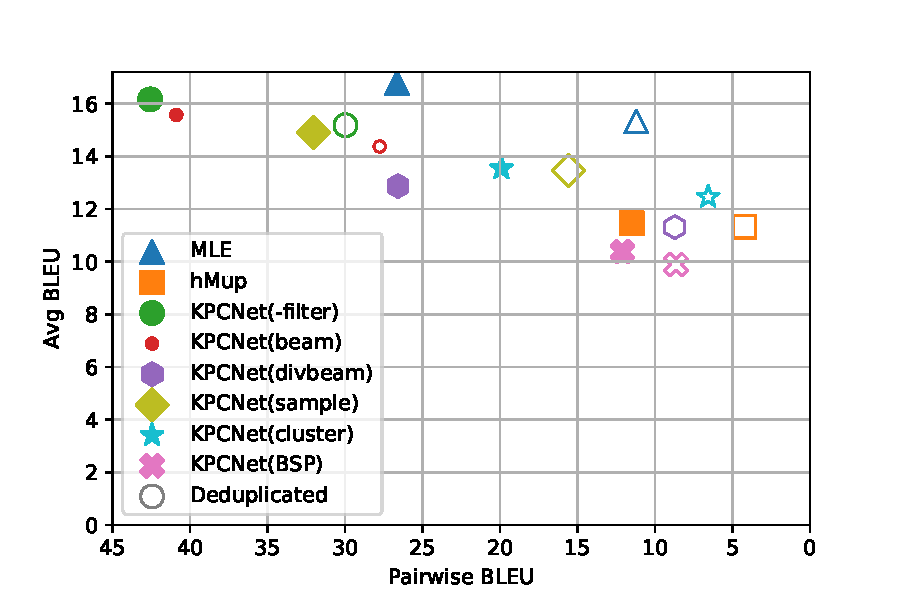
\includegraphics[width=\linewidth]{tradeoff-2BLEU.pdf}
  \caption{Group-level Automatic metrics on the whole test set of \texttt{Home \& Kitchen}. The lower Pairwise BLEU, the more diverse the generated group. Solid markers are the results for the top 3 candidates in the original group, while hollow markers measures the remaining 3 after deduplication. Points located near top-right are preferred as they achieve a good tradeoff between the 2 metrics.}
  \label{fig:group-filter}
  \end{figure}

  

\subsubsection{Group-level Evaluation}



The group-level automatic evaluation metrics before and after deduplication for each system are shown in Figure \ref{fig:group-filter}. Original results are shown in solid markers. KPCNet(BSP) has the poorest Avg BLEU and we found the results very likely to be ungrammatical and illogical, and we thus omit it in the following evaluation. hMup has the highest local diversity while has the second poorest Avg BLEU. MLE has moderate level of local diversity and the highest Avg BLEU, and we found that Keyword Filtering slightly harmed Avg BLEU, which is against our intuition. But we later found Avg BLEU doesn't correlate well with most human judgements (discuss later). Several diversity-promoting variants of KPCNet improved local diversity at the cost of Avg BLEU, among which KPCNet(cluster) achieved a best tradeoff between the two. Comparing the original and deduplicated results (hollow markers), we can see that our simple heuristic can effectively eliminate redundancy at the cost of slight degradation of Avg BLEU, as only nearly identical hypotheses with high BLEU are excluded. 

Group-level human evaluation results are shown in Table \ref{tab:group-human-eval}. We can see that all KPCNet variants clearly outperform baselines in \textit{Relevant} and \textit{Specific} while have a competitive performance in \textit{New info}. MLE rated best for \textit{Logical} for its conservative generations (low \textit{Specific}), and the questions tend to overlap with each other, as is reflected in high \textit{\#Redundant}. KPCNet(beam) has a even higher redundancy since its searching space is further limited by the conditioned keyword set. Diverse generation variants can help overcome this drawback. Especially, KPCNet(cluster) achieved the best \textit{\#Useful}, \textit{Avg Rank}, and its performance on all metrics is among the best of KPCNet variants. This shows that the semantically-coherent keyword sets produced by clustering can effectively improve the generation diversity and quality of KPCNet. 

We also study the system-level Pearson correlation between the automatic metrics and human judgements. Pairwise-BLEU has a correlation  of 0.915 with \textit{\#Redundant} ($p<0.01$), -0.835 with \textit{\#Useful} ($p<0.05$). Avg BLEU is shown only correlates well with \textit{Logical} (correlation: 0.849, $p<0.05$). This result validates the use of Pairwise-BLEU as an automatic proxy metric for local diversity.

\subsubsection{Case Study}

\begin{table*}[htbp]
  \centering
  \begin{tabular}{c|lcc}
      \hline
      product & \makecell[l]{homelegance 2588s accent dining chair, blue grey, set of 2} & {} & {} \\
      \hline
      \makecell[c]{system \\ (\#Useful)} & generation group & specific & problem \\
      \hline
      \makecell[c]{ref \\ (3)} & \makecell[l]{can any of the recent reviewers confirm the seat height ? \\ i see the question was posted in april ... \\ would u please send me the box dimensions ( when buy in \\ a set of 2 ) and the weight ? \\ can someone please tell me the depth of the chair seat \\ from the end of the curved back to the end of the seat ? } & \makecell[c]{2 \\ \\ 3 \\ \\ 3 \\ \\} & {} \\
      \hline
      \makecell[c]{MLE \\ (1)} & \makecell[l]{what is the seat height ? \\ what are the dimensions of the chair ? \\ what are the dimensions ?} & \makecell[c]{2 \\ 2 \\ 1} & {} \\
      \hline
      \makecell[c]{hMup \\ (1)} & \makecell[l]{what is the weight limit for the chair ? \\ i have a table that is a [UNK]. will this chair be able \\ to fit on a table ? \\ is this a set of 2 chairs or just one ?} & \makecell[c]{2 \\ 2 \\ \\ 2} & \makecell[c]{ \\ illogical \\ \\ repetitive} \\
      \hline
      \makecell[c]{KPCNet \\ (2)} & \makecell[l]{what is the \textbf{color} of the \textbf{chair} ? \\ what are the \textbf{dimensions} of the \textbf{seat} ? \\ what is the \textbf{weight} limit ? } & \makecell[c]{2 \\ 2 \\ 2} & \makecell[c]{ repetitive \\ \\  \\ } \\
      \hline
      \end{tabular}
      \caption{\label{table:quality} Example generation group and the human judgements for each system. Here we use KPCNet to stand for KPCNet(cluster) for brevity, and the appeared keywords of KPCNet are in bold. }
\end{table*}

\begin{table}[htbp]
  \small
  \centering
  \begin{tabular}{l|l}
  \hline
  Product & \makecell[l]{Novaform memory foam comfort curve pillow} \\
  \hline
  \makecell[l]{KPCNet \\ (cluster)} & \makecell[l]{is this a \textbf{firm} \textbf{pillow}? (pillow, foam, sleep, firm) \\ is this pillow good for \textbf{stomach sleepers}? \\ (stomach, sleeper)} \\
  \hline
  Product & \makecell[l]{full-sized headboard in solid wood} \\
  \hline
  \makecell[l]{KPCNet \\ (cluster)} & \makecell[l]{what is the height of this \textbf{headboard} ? \\ (bed frame headboard) \\ does it have a \textbf{box spring} ? (mattress box spring)} \\
  \hline
  \end{tabular}
  \caption{\label{tab:kwd-cluster} Example generation groups for KPCNet(cluster). Keywords in the parentheses.}
  \end{table}


Table \ref{tab:kwd-cluster} provides 2 example generation groups of KPCNet(cluster). For each group, the 6 predicted keywords captured specific aspects of the product. Then they are divided into 2 coherent groups (as they formed natural phrases such as ``firm pillow'' and ``stomach sleeper'') by clustering. Finally, the different conditioned keyword sets are reflected in the generation. In the first case, specific and diverse generations are successfully produced with precisely predicted keywords. We can see that the separation of keywords as controlling factors allows the novel use of classical clustering technique to help generate high-quality question groups by first producing coherent keyword sets. There are also bad cases like the second question in another group. The possible reason is that keyword predictor produced related but unsuitable keywords ``box spring'', which can be asked for a whole bed but not for headboard alone. This shows that predictor is the performance bottleneck of KPCNet.


We provide a group-level evaluation example in Table \ref{table:quality}. We can see that the diversity of MLE is very limited (it gets \textit{\#Useful} of only 1, though all 3 questions are valid, and thus \textit{\#Redundant} is 2), and it produces highly generic question. The generations are more diverse for hMup. However, we find that a certain expert of hMup has a style of long and illogical generation, like the second one demonstrated here. (It's abnormal to put chairs \textit{on} a table, and the text is not coherent as it doesn't use a pronoun in the second sentence.) This may attribute to its focus on \textit{style} instead of aspects of the products, as it is originally proposed for translation of diverse styles. This significantly harms hMup's group-level performance (Table 4) compared to its best single model (Table 3). KPCNet(cluster) produces a diverse and specific generation, and we can clearly see the effect of keyword in its generation. 

\subsection{\texttt{Office} Dataset Results}

For brevity, we only show the individual-level automatic evaluation and group-level human judgement results. All the experimental settings are the same with the previous experiments, except that we apply no keyword filtering here. 

\begin{table}[htbp]
  \centering
  \small
  \begin{tabular}{l|ccccc}
  \hline
  {} & Distinct-3 & BLEU & METEOR \\
  \hline
  ref  &        75.54 &        - &    - \\
  \hline
  MLE &        20.33 &  \textbf{14.73} & 13.81 \\
  hMup &        15.31 &  10.45 &    12.52  \\
  KPCNet &        \textbf{30.99} &     13.84 &    \textbf{15.29}  \\
  \hline
  \end{tabular}
  \caption{\label{tab:ind-auto-eval-office} Individual-level automatic evaluation results on the \texttt{Office} dataset.}
\end{table}

  
\begin{table*}[htbp]
\centering
\small
\begin{tabular}{l|ccccccc}
\hline
{} & Grammatical\tiny{[0-1]} & Relevant\tiny{[0-1]} & Logical\tiny{[0-1]} & New Info\tiny{[0-1]} & Specific\tiny{[0-4]} & \#Useful\tiny{[0-3]} & \#Redundant\tiny{[0-2]} \\
\hline
ref         &       0.993 &    0.997 &   0.993 &    0.933 &    2.713 &   2.420 &      0.330 \\
\hline
MLE         &       0.970 &    0.843 &   \textbf{0.883} &    0.797 &    1.470 &   1.070 &      0.420 \\
KPCNet &       \textbf{0.993} &    \textbf{0.940} &   0.817 &    \textbf{0.803} &    \textbf{1.903} &   \textbf{1.470} &      \textbf{0.190} \\
\hline
\end{tabular}
\caption{\label{tab:group-human-eval-office} Group-level human judgments on 100 samples from the \texttt{Office} dataset. KPCNet here uses keyword clustering.}
\end{table*}

Table \ref{tab:ind-auto-eval-office} shows that KPCNet still outperforms MLE in Distinct-3 and METEOR, while falls behind at BLEU. Both the automatic metrics and our manual check indicate that hMup fails to give comparable results for 
the small dataset, so we exclude it in group-level evaluation. 



Table \ref{tab:group-human-eval-office} shows that the performance of both models degraded here possibly due to the smaller data size. However, the observation is similar. KPCNet(cluster) outperforms MLE in most metrics especially at \textit{Relevant}, \textit{Specific} and \textit{\#Useful} despite a weakness at \textit{Logical}. This shows that KPCNet(cluster) can consistently improve the diversity and specificity of the generation.


